\documentclass[usletter]{article}
\usepackage{graphicx}
\usepackage{amsfonts}
\usepackage{amsthm}
\usepackage{amsmath}
\usepackage{amssymb}
\usepackage{scribe}
\usepackage[margin=1.5in]{geometry}

\begin{document}


\makeheader{John Bender}               % your name
           {January 6, 2014}           % lecture date
           {1}                         % lecture number
           {Deterministic Computation} % lecture title

\noindent
Using the provided \verb|\makeheader| command,
customize the above header with your name,
lecture date, lecture number, and lecture title. For
example, the above header was generated by typing
\verb|\makeheader{Ima Student}{January 9, 2012}{15}|{\tt
\{Instructions for Preparing Scribe Notes\}}.  Your
scribe notes should start with a high-level description
of the lecture, its goal and techniques, and how it
fits in the broader context of the course. In
particular, explain its relation to the previous
lecture if appropriate.  This high-level description
should be two or three solid paragraphs in length.

-

The first lecture was an introduction to deterministic computation by way of a review and formalization of different Turing machines, their properties, and how those properties affect running time. In particular we discussed the impact of restricting a Turing machine with an arbitrary but finite alphabet to a binary alphabet and also the restricting a Turing machine with bidirectional, infinite tapes to unidirectional infinite tapes. Along the way we also saw key definitions and concepts related to understanding computation using Turing machines.

\textbf{TODO} define the notation used in the equations that is not part of the definition of a Turing machine, e.g. $\rhd, \Box, \{0,1\}^*$, maybe in an appendix?

\section{Turing machines}

As explained during the lecture, the Turing machine is a remarkably robust model for computation. (why?)

We will examine what a Turing machine must have in detail but first at a high level the components are as follows:

\begin{enumerate}
  \item A finite set of ``tapes''  where the cardinality of the set is represented by $k$, and each tape has an infinite number of discrete ``cells''.
  \item $k$ ``heads'' that read and write to a single cell on each tape and also handle the movement between cells.
  \item A finite alphabet, $\Gamma$, that contains the symbols each head will write to and read from the tapes.
  \item A register that stores the current ``state'' of the Turing machine from the finite set of possible states $Q$.
  \item A transition function, $\delta$, that maps from the symbols in the $k$ cells currently under each head and the current state to symbols for the same cells, a movement (or lack thereof) for each head, and a new state.
\end{enumerate}

Diagram?

Tapes most often start as far to the left as possible. That is, most representations of the Turing machine consist of tapes that only extend to the right infinitely. As we'll see later, even those that extend in both directions can be ``reduced'' to a Turing machine that only extends infinitely in one direction. Also, the first tape is the ``input tape'' and the head for that tape is ``read-only''. That is, the transition function can never tell the head for the input tape to write or similarly must always write the same symbol back.

The heads for each tape are responsible for reading values as input to the transition function, $\delta$, and writing the output from $\delta$ to the $k-1$ ``read-write'' tapes. They are also responsible for moving the tape left one cell, right one cell, or not at all depending on the output of $\delta$. Each is represented by $\leftarrow$, $\rightarrow$, and $\cdot$ respectively in subsequent discussion. Finally, When a head attempts to move the tape right at the tape's left-most extent it will simply stay put.

The alphabet $\Gamma$ must, at a minimum, contain both the start symbol, $\rhd$, the blank symbol $\Box$ and at least two more symbols to perform any computation. $\rhd$ is used to signal to the transition function, $\delta$, when a given head is at the left-most extent of its tape. The second is normally used to signify the end of other symbols on a given tape. Most often $\Gamma$ is simply the set $\{\rhd, \Box, 0, 1\}$. Otherwise the alphabet can contain a finite number of arbitrary symbols, but as we'll discuss later it is possible ``encode'' all other alphabets using the simple one.

The state register assumes values from a the finite set $Q$ that must contain the states $\textsf{START}$ and $\textsf{HALTED}$ but is otherwise arbitrary. Some Turing machines have many registers but once again these can be encoded using the cartesian product of each set of possible values for the individual registers [1].

Finally, the transition function, $\delta$,

\textbf{TODO} provide the definition, show the full example from the lecture as an introduction. Include a sample table definitions for $\delta$ for the lecture example. Full $\delta$? Note about delta being a total function though that appears to be implicit in the definition of function, ie you only qualify things as partial functions.




\section{Organization}
Lecture proper should be presented in a sequence of
sections. For example, you might choose to present
preparatory work in one section, the main results in
another section, and any generalizations or conclusions
in a third section. Do \emph{not} use any subdivisions
within sections (subsections, subsubsections, etc.).
Use normal capitalization in section headings rather
than initial caps.

\section{Some do's}
The single most important thing to keep in mind when
preparing scribe notes is that they should be a
self-contained record of the lecture.  In
particular, it is wholly inadequate to simply typeset
the contents of the blackboard---such an ``effort'' will
be rewarded with a flat grade of 1 point.  The lecture
is much more than the contents of the
blackboard; I do not just walk in the classroom and
write on the blackboard for two hours. The lecture has
a \emph{soundtrack}, which supplies a motivation for
the material, intuitive descriptions of the proofs, and
answers to questions from the audience.  This component
of the lecture is vital to understanding the subject
matter and should be prominently present in your scribe
notes.  Here are some other things to keep in mind.

\begin{itemize}
\item Always preface a formal statement (theorem,
lemma, proposition) with a discussion of its purpose
and a brief and intuitive outline of the proof.

\item We all know from experience that a picture is
worth a thousand words, so be generous with figures.
Please be sure to include all the figures and drawings
from my lecture, and feel free to include your own. See
Figure~\ref{fig:triangle-circle} for an example usage
of the figure environment.

\item Write in complete sentences.  Mathematical
writing is not fundamentally different from any other
form of expository prose. Take pride in your work.

\item As with any writing, make sure to spell check
your scribe notes.

\item Be sure to include all bibliographic references,
like so~\cite{textbook}. You will find all the needed
references at the end of the corresponding chapter in the
textbook. The bibliography must be incorporated using
BibTex.  When finished, please send me the following
files by email: your \LaTeX\ source file ({\tt .tex}),
your bibliography file ({\tt .bib}) if you used one,
any figures (ideally in {\tt .pdf} format), and the
resulting typeset document ({\tt .pdf}).   I prefer to
receive a single ZIP archive rather than several
individual attachments.
\end{itemize}

\begin{figure}
\begin{center}
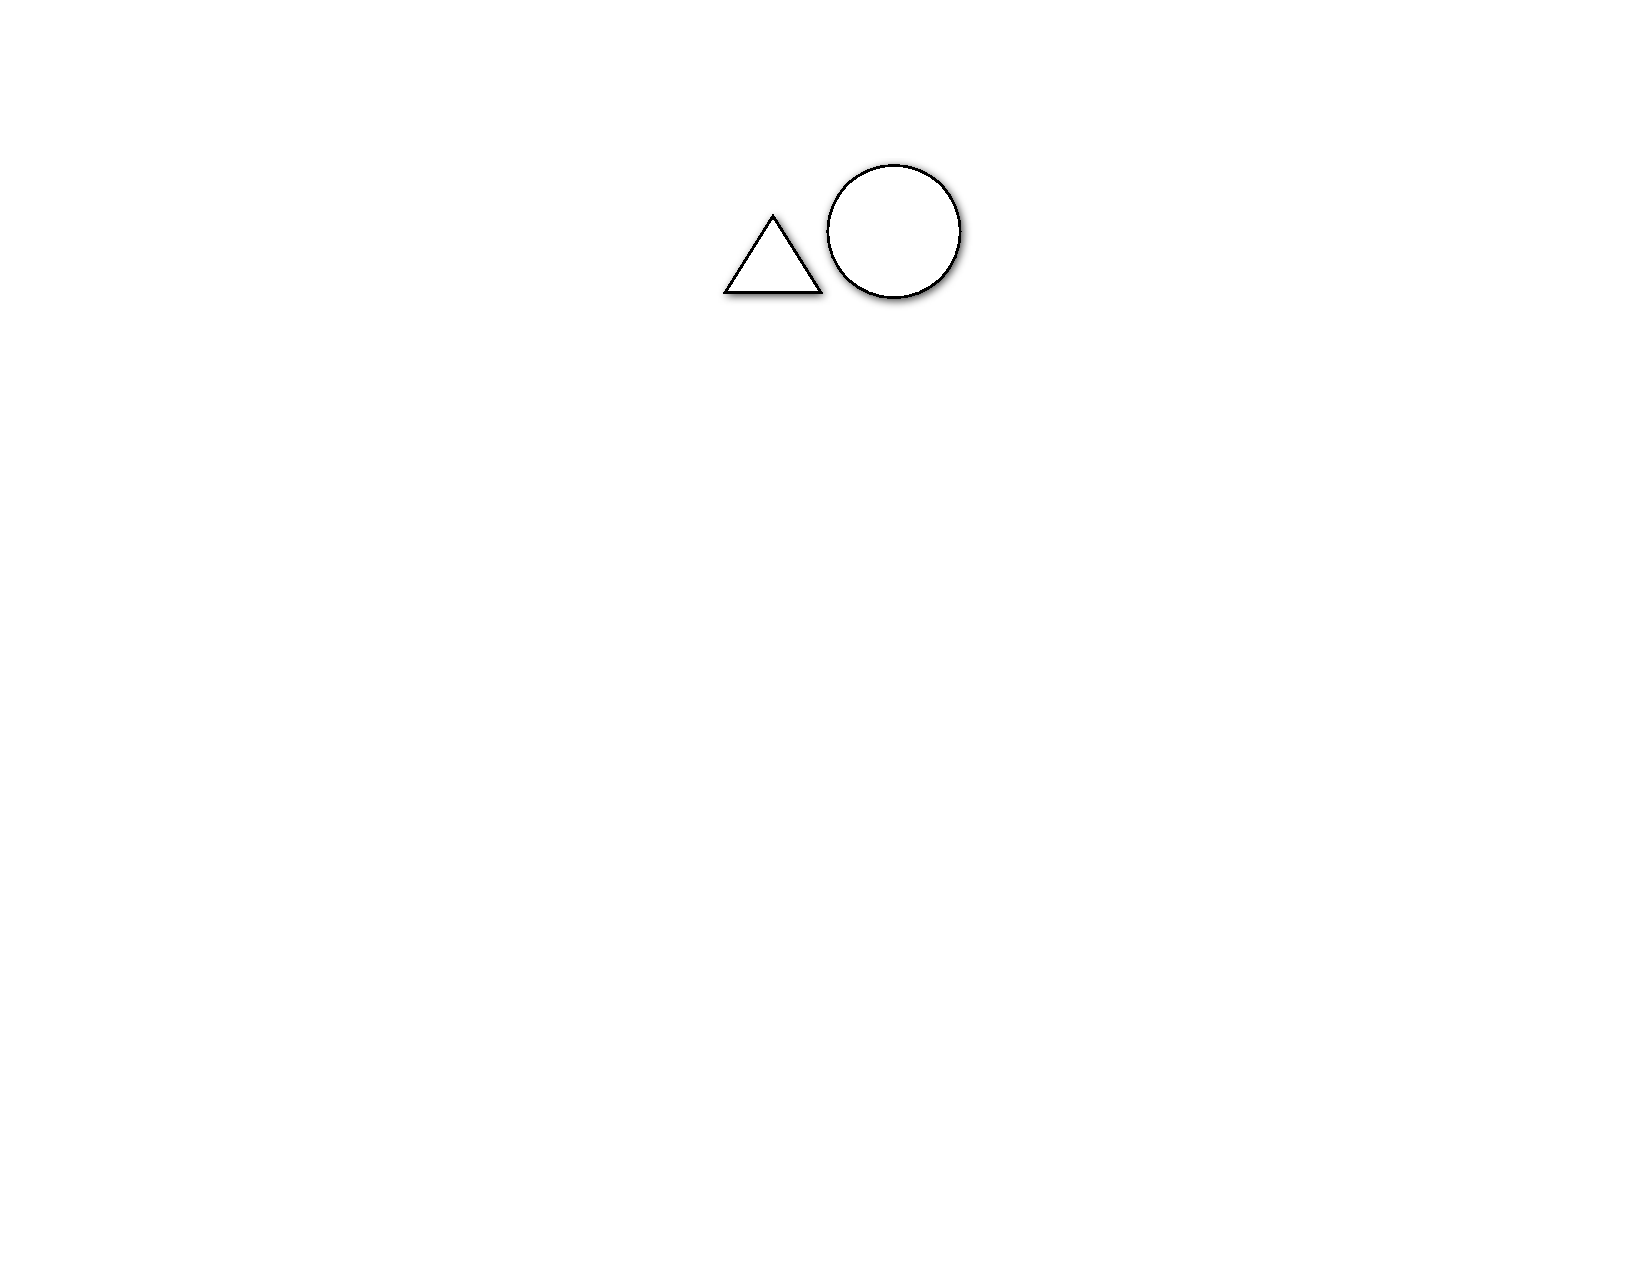
\includegraphics[width=0.4\textwidth]{triangle-circle}
\end{center}
\caption{A triangle and a circle.}
\label{fig:triangle-circle}
\end{figure}

\section{Some don'ts}

Here are the most common pitfalls to watch out for.

\begin{itemize}
\item Copying or paraphrasing material from the
textbook is emphatically \emph{not} OK because it
defeats the pedagogical purpose of scribe notes.  What
I am looking for is \emph{your} personal perspective on
the material. A good way to proceed is to master the
material from the lecture and textbook, wait a day
for it to sink in, and then typeset your scribe notes
without consulting any sources. This approach brings
out your personal take on the material and allows you
to truly internalize it to a point when you yourself
could teach it.

\item You must not change the format of the scribe
notes in any way, including font type, font size,
pagination, section numbering, margins, or bibliography
style.

\item No content should spill over into the margins.

\item You must not use any \LaTeX\ packages that do not
come with the standard \LaTeX\ installation in our
department; as a matter of fact, you should not need to
include any \LaTeX\ packages in addition to those
already included in the template file.
\end{itemize}


\section{Mathematical environments}

For your convenience, the scribe note style file comes
with the following mathematical environments
predefined: theorem, lemma, corollary, proposition,
fact, claim, definition, example, assumption, remark,
conjecture, open problem, problem. The environments are
illustrated below.  Please limit yourself to these
environments.

\begin{theorem}
Statement here
\end{theorem}

\begin{lemma}
Statement here
\end{lemma}

\begin{corollary}
Statement here
\end{corollary}

\begin{proposition}
Statement here
\end{proposition}

\begin{fact}
Statement here
\end{fact}

\begin{claim}
Statement here
\end{claim}

\begin{definition}
Statement here
\end{definition}

\begin{example}
Statement here
\end{example}

\begin{assumption}
Statement here
\end{assumption}

\begin{remark}
Statement here
\end{remark}

\begin{conjecture}
Statement here
\end{conjecture}

\begin{openproblem}
Statement here
\end{openproblem}

\begin{problem}
Statement here
\end{problem}


\noindent
Note that \LaTeX\ automatically numbers these
environments within the lecture number (\thelecture\ in
this case).  The same applies to the numbering of pages
(this page being page \thepage), figures
(Figure~\ref{fig:triangle-circle} above), and
equations:
\begin{align}
a = a_1+a_2+\cdots+a_n.
\end{align}
\noindent
For proofs, use the provided {\tt proof} environment,
illustrated below.

\begin{proof}
Proof goes here.
\end{proof}


\bibliographystyle{abbrv}
\bibliography{template}

\end{document}
